\documentclass[9pt]{beamer}

% Theme choice:
\usetheme{CambridgeUS}

%Packages
\usepackage[backend=biber,hyperref=true,doi=false,url=false,isbn=false, uniquename=false, uniquelist=false, style = authoryear-comp]{biblatex}
%https://www.overleaf.com/learn/latex/Biblatex_citation_styles
\addbibresource{synthVolForecast.bib}

%\usepackage{bibentry}

\usepackage{graphicx}
\usepackage{amsmath}
\usepackage{amsfonts}
\usepackage{amsthm}
\usepackage[export]{adjustbox}
\usepackage{amssymb}
\usepackage[useregional]{datetime2}
\usepackage{verbatim}
\usepackage{mathtools}% http://ctan.org/pkg/mathtools
\usepackage{mathrsfs}


\usepackage{amscd}
\usepackage{url}
% \usepackage[table,xcdraw,usenames]{xcolor}
% \usepackage[usenames]{color}

\usepackage{subcaption}
% \usepackage{enumitem}
% \usepackage{authblk}
% \usepackage{bm}
% \usepackage{pdfpages}

\usepackage{hyperref}
\usepackage{caption}
\usepackage{float}
%\usepackage[caption = false]{subfig}
\usepackage{tikz}
\usepackage{multirow}
\usepackage[linesnumbered, ruled,vlined]{algorithm2e}
\usepackage{pdflscape}
\usepackage{etoolbox}

%\AtBeginEnvironment{align}{\setcounter{equation}{0}} % https://tex.stackexchange.com/questions/349247/how-do-i-reset-the-counter-in-align

% function definition
\newcommand{\weight}{\pi}
\newcommand{\V}{\textbf{V}}
\newcommand{\ret}{\textbf{r}}
\newcommand{\y}{\textbf{y}}
\newcommand{\w}{\textbf{w}}
\newcommand{\x}{\textbf{x}}
\newcommand{\dbf}{\textbf{d}}
\newcommand{\X}{\textbf{X}}
\newcommand{\Y}{\textbf{Y}}
% \newcommand{\L}{\textbf{L}}
\newcommand{\Hist}{\mathcal{H}}
\newcommand{\Prob}{\mathbb{P}}
\def\mbf#1{\mathbf{#1}} % bold but not italic
\def\ind#1{\mathrm{1}(#1)} % indicator function
\newcommand{\simiid}{\stackrel{iid}{\sim}} %[] IID
\def\where{\text{ where }} % where
\newcommand{\indep}{\perp \!\!\! \perp } % independent symbols
\def\cov#1#2{\mathrm{Cov}(#1, #2)} % covariance
\def\mrm#1{\mathrm{#1}} % remove math
\newcommand{\reals}{\mathbb{R}} % Real number symbol
\def\t#1{\tilde{#1}} % tilde
\def\normal#1#2{\mathcal{N}(#1,#2)} % normal
\def\mbi#1{\boldsymbol{#1}} % Bold and italic (math bold italic)
\def\v#1{\mbi{#1}} % Vector notation
\def\mc#1{\mathcal{#1}} % mathical
\DeclareMathOperator*{\argmax}{arg\,max} % arg max
\DeclareMathOperator*{\argmin}{arg\,min} % arg min
\def\E{\mathbb{E}} % Expectation symbol
\def\mc#1{\mathcal{#1}}
\def\var#1{\mathrm{Var}(#1)} % Variance symbol
\def\checkmark{\tikz\fill[scale=0.4](0,.35) -- (.25,0) -- (1,.7) -- (.25,.15) -- cycle;} % checkmark
\newcommand\red[1]{{\color{red}#1}}
\def\bs#1{\boldsymbol{#1}}
\def\P{\mathbb{P}}
\def\var{\mathbf{Var}}
\def\naturals{\mathbb{N}}
\def\cp{\overset{p}{\to}}
\def\clt{\overset{\mathcal{L}^2}{\to}}

\setcounter{tocdepth}{4}
\setcounter{secnumdepth}{4}

\newcommand{\ceil}[1]{\lceil #1 \rceil}
\newcommand{\norm}[1]{\left\lVert#1\right\rVert} % A norm with 1 argument
\DeclareMathOperator{\Var}{Var} % Variance symbol

\newtheorem{cor}{Corollary}
\newtheorem{lem}{Lemma}
\newtheorem{thm}{Theorem}
\newtheorem{defn}{Definition}
\newtheorem{prop}{Proposition}
\theoremstyle{definition}
\newtheorem{remark}{Remark}
\hypersetup{
  linkcolor  = blue,
  citecolor  = blue,
  urlcolor   = blue,
  colorlinks = true,
} % color setup

% % \makeatletter
% % \setbeamertemplate{footline}
% % {
% %     \leavevmode%
% %     \hbox{%
% %         \begin{beamercolorbox}[wd=.333333\paperwidth,ht=2.25ex,dp=1ex,center]{author in head/foot}%
% %             \usebeamerfont{author in head/foot}\insertshortauthor
% %         \end{beamercolorbox}%
% %         \begin{beamercolorbox}[wd=.333333\paperwidth,ht=2.25ex,dp=1ex,center]{title in head/foot}%
% %             \usebeamerfont{title in head/foot}\insertshorttitle
% %         \end{beamercolorbox}%
% %         \begin{beamercolorbox}[wd=.333333\paperwidth,ht=2.25ex,dp=1ex,right]{date in head/foot}%
% %             \usebeamerfont{date in head/foot}\insertshortdate{}\hspace*{2em}
% %             \insertframenumber{} / \inserttotalframenumber\hspace*{2ex}
% %         \end{beamercolorbox}}%
% %         \vskip0pt%
% %     }
% %     \makeatother

\title{Synthetic Volatility Forecasting and Other Aggregation Techniques for Time Series Forecasting}
\subtitle{Preliminary Exam}
\author{David Lundquist\thanks{davidl11@ilinois.edu}, Daniel Eck\thanks{dje13@illinois.edu} (advisor)}
\date{April 10th, 2024}

\begin{document}

\part{one}
%% title frame
\begin{frame}
\titlepage
\end{frame}

\section{Introduction}

\begin{frame}
\frametitle{A seemingly unprecedented event might make one ask}
\begin{enumerate}
    \item <1-> What does it resemble from the past?
    \item <2-> What past events are most relevant for our objectives?
    \item <3-> Can we incorporate past events in a systematic, principled manner?
\end{enumerate}
\end{frame}

\begin{frame}
    \frametitle{When would we ever have to do this?}

    \begin{itemize}
        \item <1-> Event-driven investing strategies (unscheduled news shock)
        \item <2-> Pairs trading strategies
        \item <3-> Scheduled macroeconomic news possibly pre-empted by a news leak
        

        \href{https://www.wsj.com/articles/bad-inflation-reports-raise-odds-of-surprise-0-75-percentage-point-rate-rise-this-week-11655147927}{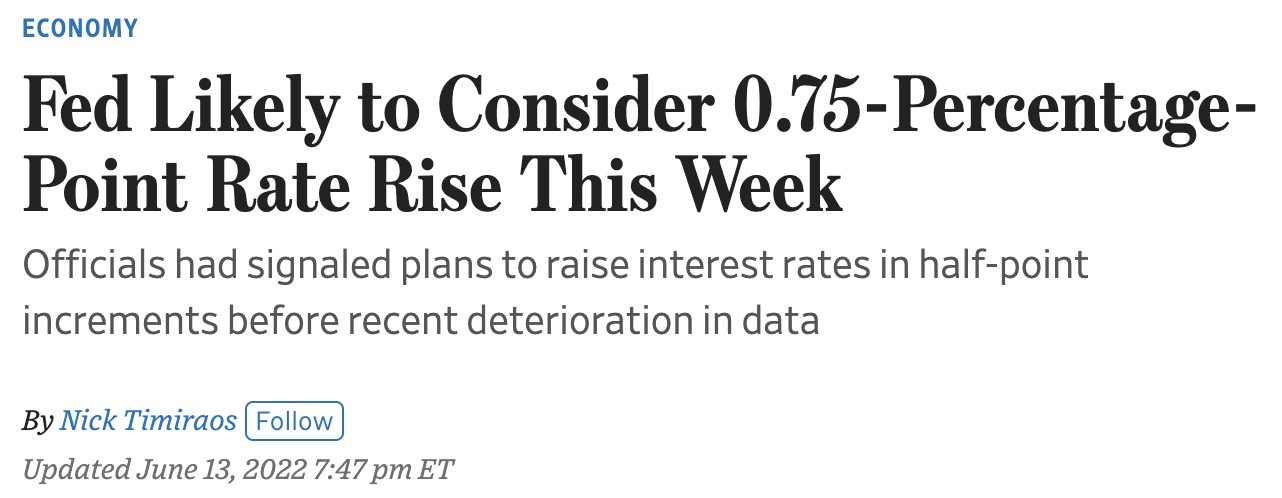
\includegraphics[scale=.3]{WSJ_rate_hike_2022.png}}
    \end{itemize}
\end{frame}

\begin{frame}

    \begin{example}[Weekend of March 6th - 8th, 2020]
        \href{https://www.governor.ny.gov/news/novel-coronavirus-briefing-governor-cuomo-declares-state-emergency-contain-spread-virus}{
\includegraphics[scale=.3]{NYS_state.png}}

        \href{https://www.cnbc.com/2020/03/08/opec-deal-collapse-sparks-price-war-20-oil-in-2020-is-coming.html}{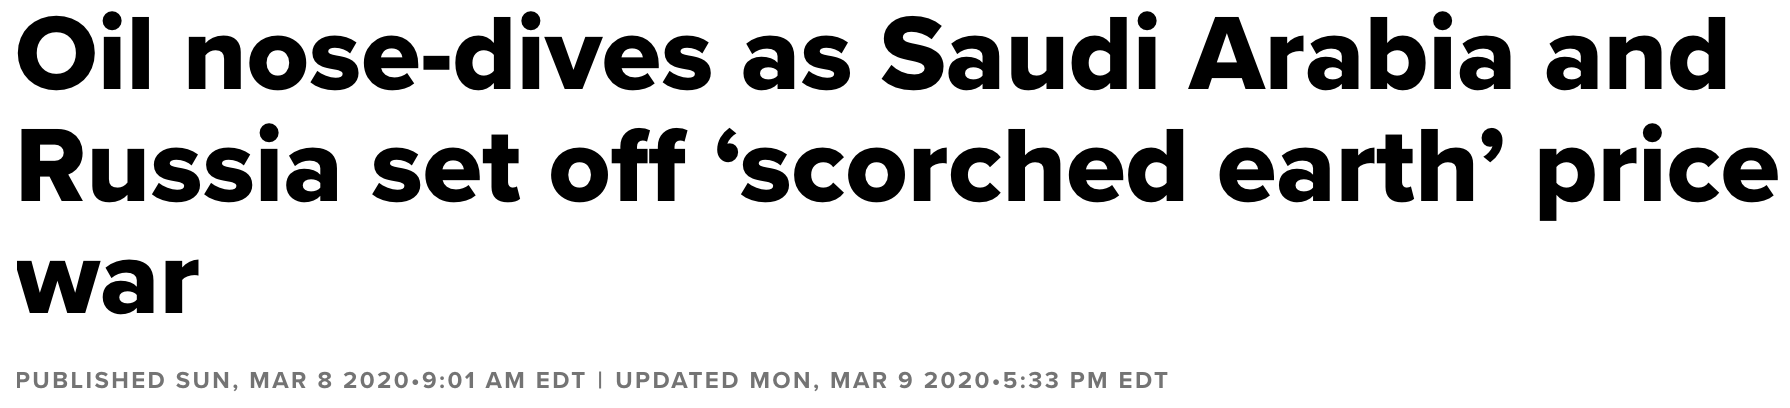
\includegraphics[scale=.3]{cnn.png}}

        \href{https://www.cnn.com/2020/03/08/investing/oil-prices-crash-opec-russia-saudi-arabia/index.html}{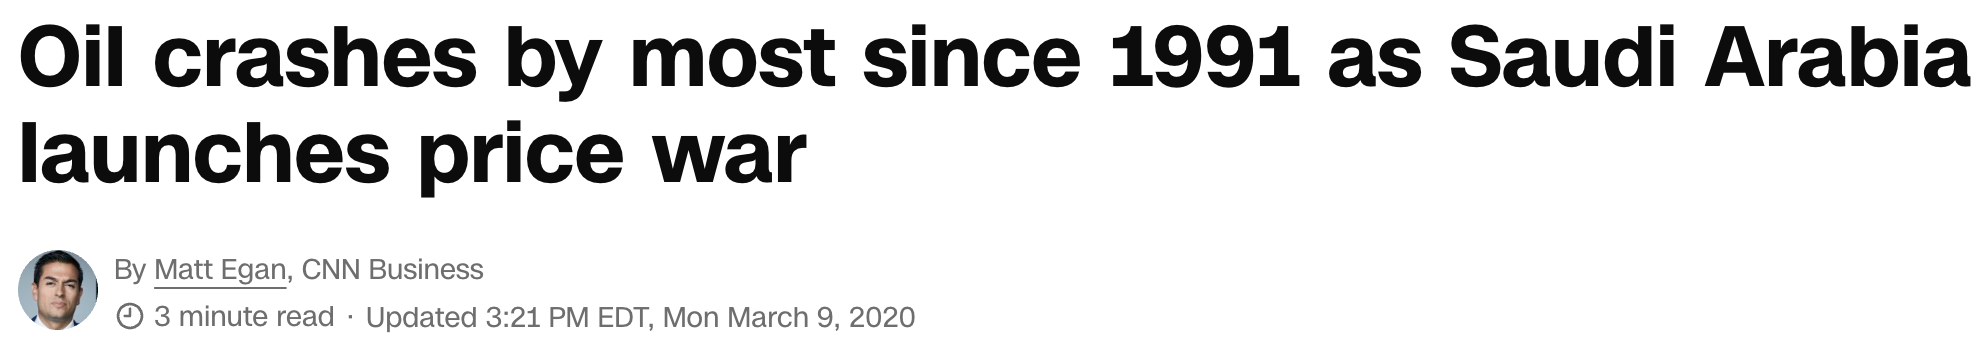
\includegraphics[scale=.3]{cnbc.png}}
        \end{example}

\end{frame}

\begin{frame}
\frametitle{Punchline of the paper}

\begin{itemize}
    \item[] <1-> Credible forecasting is possible under news shocks, so long as we incorporate external information to account for the \textcolor{red}{nonzero errors}.
    \item[] <2-> \begin{figure}[H]
        \begin{center}
          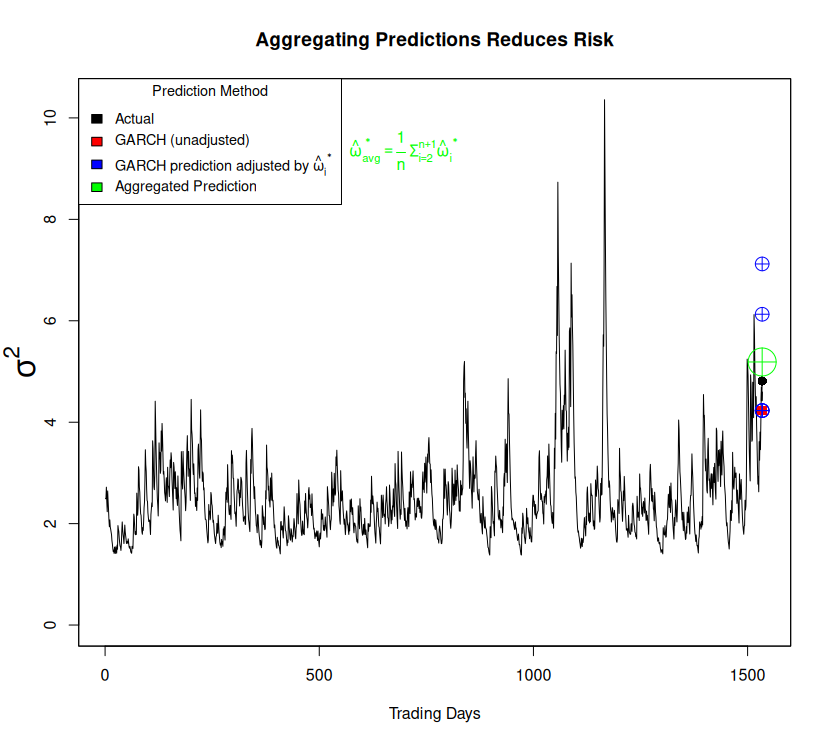
\includegraphics[scale=.3]{simulation_plots/alternative_USE_in_paper_simulation_plot_arithmetic_mean.png}
          \caption{Adjusting our One-Step-Ahead Forecast Using Only Arithmetic Mean of Donors}
          \end{center}
        \end{figure}
\end{itemize}
\end{frame}

\begin{frame}
    \frametitle{Background and related methods}
    Volatility Modeling

    \begin{itemize}
        \item GARCH is slow to react to shocks \parencite[][]{andersen2003modeling}
        \item Asymmetric GARCH models catch up faster but need post-shock data
        \item Realized GARCH \parencite[][]{hansen2012realized}, in our setting, would require post-shock information and/or high-frequency data in order to outperform, and Realized GARCH is highly parameterized
    \end{itemize}
\end{frame}

\begin{frame}
    \frametitle{Background and related methods}

    Forecast Adjustment
    \begin{itemize}
        \item \cite[][]{clements1996intercept,clements1998forecasting} laid the groundwork for modeling nonzero errors in time series forecasting
        \item \cite[][]{guerron2017macroeconomic} use a series' own errors to correct the forecast for that series
        \item \cite[][]{dendramis2020similarity} use a similarity-based procedure to correct $\hat\beta$ in time series forecasts
        \item \cite[][]{foroni2022forecasting} adjust pandemic-era forecasts using intercept correction techniques and data from Great Financial Crisis
        \item \cite[][]{lin2021minimizing} use distanced-based weighting (a similarity approach) to aggregate and weight fixed effects from a donor pool
    \end{itemize}
\end{frame}

\part{two}
\section{Setting}
% Outline frame
\begin{frame}{Outline} % https://tex.stackexchange.com/questions/73196/beamer-table-of-contents-shade-all-previous-sections
    \tableofcontents[part=1,currentsection]\tableofcontents
\end{frame}

% Presentation structure

% Setting for the problem
\begin{frame}
\frametitle{Premise: News has broken but markets are closed}

\begin{itemize}
\item After-hours trading provides a poor forum in which to digest news
\item News constitutes public, material information for one or more traded assets
\item The \textcolor{red}{qualitative aspects} of the news provide a basis upon which to 
\begin{itemize}
    \item match to past news shocks
    \item match in a $p$-dimensional covariate space
\end{itemize}
\end{itemize}
\end{frame}

\begin{frame}
    \frametitle{A Primer on GARCH}
   
    \begin{Definition}

    Let $\{a_{t}\}$ denote an observable, real-valued discrete-time stochastic process.\\
    
    \bigbreak
    
    We call $\{a_{t}\}$ a strong GARCH process \parencite[][]{francq2019garch} with respect to $\{\epsilon_{t}\}$ iff 
    \begin{align*}
        &\sigma_{t}^{2} = \omega + \sum^{m}_{k=1}\alpha_{k}a^{2}_{t-k} + \sum_{j=1}^{s}\beta_{j}\sigma_{t-j}^{2}\\
        &a_{t} = \sigma_{t}\epsilon_{t}\\
        &\epsilon_{t} \simiid E[\epsilon_{t}]=0, Var[\epsilon_{t}] = 1\\
        &\forall k,j, \alpha_{k},\beta_{j}\geq 0\\ 
        &\forall t, \omega, \sigma_{t} > 0 
        \end{align*}

    \end{Definition}

\end{frame}

\begin{frame}
    \frametitle{Volatility Equation with an exogenous term: GARCH-X}
    
    \begin{align*}
        &\sigma_{t}^{2} = \omega+ \sum^{m}_{k=1}\alpha_{k}a^{2}_{t-k} + \sum_{j=1}^{s}\beta_{j}\sigma_{t-j}^{2} + \gamma^{T}\x_{t} \text{ .}\label{GARCH-X}
    \end{align*}

    We will be looking at only one exogenous term.

    \end{frame}
    
\begin{frame}
    \frametitle{Model Preliminaries}

    \fontsize{8}{7.2}

    Let $I(\cdot)$ be an indicator function.  \\
\bigbreak
    Let $T_i$ denote the time length of the time series $i$ for $i = 1, \ldots, n+1$.\\
    \bigbreak
    Let $T_i^*$ denote the largest time index prior to news shock, with $T_i^* < T_i$ (i.e. we assume at least one post-shock observation). \\
    \bigbreak
    Let $\delta, \textbf{v}_{i,t} \in \mathbb{R}^{p},  \x_{i,t} \in \mathbb{R}^{d}$.  
\end{frame}

\begin{frame}
\frametitle{Model Setup}

\fontsize{6}{7.2}

For $t= 1, \ldots, T_i$ and $i = 1, \ldots, n+1$, the model $\mc{M}_1$ is defined as 
\begin{align*}
  \mc{M}_1 \colon \begin{array}{l}
     \sigma^{2}_{i,t} = \omega_{i} + \omega^{*}_{i,t} + \sum^{m_{i}}_{k=1}\alpha_{i,k}a^{2}_{i,t-k} + \sum_{j=1}^{s_{i}}\beta_{i,j}\sigma_{i,t-j}^{2} + \gamma_{i}^{T} \x_{i,t} \text{ }\\[.2cm]
     a_{i,t} = \sigma_{i,t}((1-D^{return}_{i,t})\epsilon_{i,t} + D^{return}_{i,t}\epsilon^{*}_{i})\\[.2cm]
    \omega_{i,t}^{*} = D^{vol}_{i,t}[\mu_{\omega^{*}}+\delta'\textbf{v}_{i, t}+ u_{i,t}],
  \end{array}
  \end{align*}\label{model_1}
with error structure

  \begin{align*}
    \epsilon_{i,t} &\simiid \mc{F}_{\epsilon} \text{ with }  \; \mrm{E}_{\mc{F}_{\epsilon}}(\epsilon) = 0, \mrm{Var}_{\mc{F}_{\epsilon}}(\epsilon)  = 1  \\
    \epsilon^{*}_{i,t} &\simiid \mc{F}_{\epsilon^{*}} \text{ with }  \; \mrm{E}_{\mc{F}_{\epsilon^{*}}}(\epsilon) = \mu_{\epsilon^{*}}, \mrm{Var}_{\mc{F}_{\epsilon^{*}}}(\epsilon^{*})  = \sigma^2_{\epsilon^{*}}  \\
    u_{i,t} & \simiid  \mc{F}_{u} \text{ with }  \; \mrm{E}_{\mc{F}_{u}}(u) = 0, \mrm{Var}_{\mc{F}_{u}}(u) = \sigma^2_{u}\\
    \epsilon_{i,t} & \indep  \epsilon^{*}_{i,t}  \indep u_{i,t}
    \end{align*}
where $D^{return}_{i,t} = I(t \in \{T_i^* + 1,...,T_i^* + L_{i, return}\})$ and $D^{vol}_{i,t} = I(t \in \{T_i^* + 1,...,T_i^* + L_{i, vol}\})$ and $L_{i,return},L_{i,vol}$ denote lengths of log return and volatility shocks, respectively.  

\bigbreak

\textcolor{red}{Note: we will be looking GARCH(1,1) only in this presentation.}
\end{frame}


% \begin{frame}
%     \frametitle{Model Details}
%     Let $\mc{M}_{0}$ denote the subclass of $\mc{M}_{1}$ models such that $\delta \equiv 0$.  \\
%     \bigbreak
%     $\mc{M}_{0}$ assumes $\omega^{*}_{i,t}$ have no dependence on the covariates and are i.i.d. with $\E[ \omega^{*}_i]=\mu_{\omega^{*}}$.  
% \end{frame}

\begin{frame}
\frametitle{Our Model is Nested inside a Factor Model}

\fontsize{6}{7.2}

Consider $\mc{M}_{1}$ in the context of the factor model from \cite[][]{abadie2010synthetic}, where an untreated unit is governed by:

$$Y^{N}_{i,t} = \delta_{t} + \boldsymbol\theta_{t}^{'}\textbf{Z}_{i}+\boldsymbol\lambda_{t}^{'}\boldsymbol\mu_{i}+\varepsilon_{i,t}$$

which nests the GARCH model's volatilty equation as well as the ARMA representation of a GARCH model, where

\begin{align*}
\delta_{t} & \sim \omega, \text{a location parameter shared across donors}\\
\boldsymbol\theta_{t} & \sim \boldsymbol\alpha_{k}, \text{a vector of ARCH parameters and other coefficients shared across donors} \\
\textbf{Z}_{i} & \sim \boldsymbol a_{i,t-k}, \text{a vector of observable quantities specific to each donor} \\
\boldsymbol \lambda_{t} & \sim \boldsymbol\beta_{j}, \text{a vector of GARCH parameters shared across donors} \\
\boldsymbol \mu_{i} & \sim \boldsymbol \sigma_{i,t-j}^{2}, \text{a vector of latent quantities specific to each donor}   \\
\end{align*}

% and $\varepsilon_{i,t}$ is idiosyncratic noise, uncorrelated across time and donors.
\end{frame}


\begin{frame}
\frametitle{Volatility Profile of a Time Series}
\fontsize{6.6}{7}

Consider the $p \times n$ matrix that stores donor and covariate information at time $t$

\begin{equation*}
    \V_{t} = 
    \begin{pmatrix}
    \hat\alpha_{1,t} & \hat\alpha_{t,2}  & \cdots & \hat\alpha_{t,n}  \\
    \hat\beta_{1,t} & \hat\beta_{t,2}  & \cdots & \hat\beta_{t,n}  \\
    \vdots  & \vdots  & \ddots & \vdots  \\
    RV_{1,t} & RV_{2,t}  & \cdots & RV_{n,t}  \\
    RV_{1,t-1}  & RV_{2,t-1}  & \cdots & RV_{n,t-1}  \\
    \vdots  & \vdots  & \ddots & \vdots  \\
    IV_{1,t} & IV_{2,t} & \cdots & IV_{n,t} \\
    IV_{1,t-1}  & IV_{2,t-1}  & \cdots & IV_{n,t-1} \\
    \vdots  & \vdots  & \ddots & \vdots  \\
    |r_{1,t}| & |r_{2,t}| & \cdots & |r_{n,t}| \\
    |r_{1,t-1}|  & |r_{2,t-1}|  & \cdots & |r_{n,t-1}| \\
    \end{pmatrix},
    \end{equation*}
    \bigbreak
    where RV denotes realized variance and IV the implied volatility
\end{frame}

\begin{frame}
    \frametitle{Significance of the Volatility Profile}
    Covariates chosen for inclusion in a given volatility profile may be any $\mathcal{F}_{t}$-measurable function, for example
    \begin{itemize}
        \item levels
        \item differences in levels
        \item log returns
        \item percentage returns
        \item measurable transformations of the above
    \end{itemize}

    \bigbreak 

    Key criterion for inclusion: how plausible is the covariate as a \textcolor{red}{proxy for risk conditions} for the volatility series to be forecasted?
\end{frame}

\section{Post-shock Synthetic Volatility Forecasting Methodology}

\begin{frame}
\frametitle{Forecasting}

\fontsize{7.6}{7}

We present two forecasts:

\begin{align*}
  \text{Forecast 1: } & \hat\sigma^{2}_{unadjusted} = \hat\E[\sigma^{2}_{1,T_{1}^{*}+1}|\mathcal{F}_{T^{*}}] = \hat\omega_{i} + \sum^{m_{i}}_{k=1}\hat\alpha_{i,k}a^{2}_{i,t-k} + \sum_{j=1}^{s_{i}}\hat\beta_{i,j}\sigma_{i,t-j}^{2} + \hat\gamma_{i}^{T} \x_{i,t}\\
  \text{Forecast 2: } & \hat\sigma^{2}_{adjusted} = \hat\E[\sigma^{2}_{1,T_{1}^{*}+1}|\mathcal{F}_{T^{*}}] + \textcolor{red}{\hat\omega^{*}} = \hat\omega_{i} + \sum^{m_{i}}_{k=1}\hat\alpha_{i,k}a^{2}_{i,t-k} + \sum_{j=1}^{s_{i}}\hat\beta_{i,j}\sigma_{i,t-j}^{2} + \hat\gamma_{i}^{T} \x_{i,t} + \textcolor{red}{\hat\omega^{*} } \text{ .}
\end{align*}
\end{frame}

\begin{frame}
\frametitle{Excess Volatility Estimators}

\begin{itemize}

\item <1->  Observe the pair $(\{\hat\omega^{*}_{i}\}^{n+1}_{i=2},\{\textbf{v}_{i}\}^{n+1}_{i=2})$.  \\

\item <2-> Goal: recover weights $\{\weight_{i}\}^{n+1}_{i=2} \in \Delta^{n}$ and compute $\hat\omega^{*} \coloneq \sum^{n+1}_{i=2}\weight_{i}\hat\omega^{*}_{i}$, our forecast adjustment term.

\item <3-> Following \cite[][]{abadie2003economic,abadie2010synthetic}, let $\|\cdot\|_{\textbf{S}}$ denote any semi-norm on $\mathbb{R}^{p}$, and define


\begin{align*}
\{\pi\}_{i=2}^{n+1} = \argmin_{\pi}\|\textbf{v}_{1,T^{*}} - \V_{T^{*}}\pi \|_{\textbf{S}} \text{ .}
\end{align*}

% Nota bene: the weights $\{\weight_{i}\}_{i=2}^{n+1}$ are deterministic with respect to $\mathcal{F}_{T^{*}}$.


\end{itemize}


\end{frame}

\begin{frame}
\frametitle{Ground Truth Estimators}

We use realized volatility (RV)
\begin{itemize}
\item ``model-free'' in the sense that it requires no modeling assumptions \parencite[][]{andersen2010stochastic}.  
\item RV can be decomposed into the sum of a \textcolor{red}{continuous component} and a \textcolor{red}{jump component}, with the latter being less predictable and less persistent \parencite[][]{andersen2007roughing}, cited in \cite[][]{de2006forecasting}, two facts that further motivate our method.
\end{itemize}

\end{frame}

\begin{frame}
    \frametitle{Realized Volatility Estimation}

Examine $K$ units of of time; each unit is divided into $m$ intervals of length $\frac{1}{m}$.  Let $p_{t} = \log{P_{t}}$, and let $\tilde{r}(t,\frac{1}{m}) = p_{t} - p_{t-\frac{1}{m}}$  \parencite[][]{andersen2009realized}. 

\bigbreak

Estimate variance of $i$th log return series using Realized Volatility of the $K$ consecutive trading days that conclude with day $t$, denoted $RV_{i,t}^{K,m}$, using

$$RV_{i,t}^{K,m} = \frac{1}{K}\sum^{Km}_{v=1}\tilde{r}^{2}(v/m,1/m),$$

where the $K$ trading days have been chopped into $Km$ equally-sized blocks.

Assuming the $K$ units $\tilde{r}(t, 1) = p_{t} - p_{t-1}$ are s.t. $\tilde{r}(t, 1) \simiid N(\mu, \delta^{2})$, it is easily verified that 

$$\E[RV^{K,m}] = \frac{\mu^{2}}{m} + \delta^{2},$$
which is a biased but consistent estimator of the variance.  We pick $m = 77$, corresponding to the 6.5-hour trading day chopped into 5-minute blocks, omitting first five-minutes of the day.

\end{frame}

\begin{frame}
\frametitle{Loss Functions}

Aim: point forecasts for $\sigma^{2}_{1,T^{*}+h}|\mathcal{F}_{T^{*}}$, $h=1,2,...,$, the $h$-step ahead conditional variance for the time series under study\\

\bigbreak
 
Let $L^{h}$ with the subscripted pair $\{$prediction method, ground truth estimator$\}$, denote the loss function for an $h$-step-ahead forecast using a given prediction function and ground truth estimator.  

\end{frame}

\begin{frame}
    \frametitle{Loss Function Examples}
For example, one loss possible function of interest in this study is the 1-step-ahead MSE using Synthetic \textcolor{red}{Volatility Forecasting} and \textcolor{red}{Realized Volatility}:

$$\text{MSE}^{1}_{\text{SVF, RV}} = (\hat\sigma^{2}_{SVF} - \hat\sigma^{2}_{RV})^{2}$$
Also of interest in mean absolute percentage error for an $h$-step-ahead forecast, defined as

$$\text{MAPE}^{h}_{method, ground truth} = \frac{|\hat\sigma^{2}_{h, method} - \hat\sigma^{2}_{h, ground truth}|}{\hat\sigma^{2}_{h, ground truth}}$$

\end{frame}

\begin{frame}\frametitle{Our choice of Loss Function}

    Finally, we introduce the QL (quasi-likelihood) Loss \parencite[][]{brownlees2011practical}:

    $$\text{QL}^{h}_{method, ground truth} = \frac{ \hat\sigma^{2}_{h, method} }{\hat\sigma^{2}_{h, ground truth}} - \log{\frac{ \hat\sigma^{2}_{h, method} }{\hat\sigma^{2}_{h, ground truth}}} -1 \text{ .}$$
    
What distinguishes QL Loss? \\

\begin{itemize}

\item Multiplicative rather than additive  

\item As \cite[][]{brownlees2011practical} explain, ``[a]mid volatility turmoil, large MSE
losses will be a consequence of high volatility without necessarily corresponding to deterioration of forecasting ability. The QL avoids this ambiguity, making it easier to compare losses across volatility regimes."

\end{itemize}

\end{frame}

\section{Properties of Volatility Shock and Shock Estimators}\label{SVF_properties}

\begin{frame}\frametitle{Two Consistency Results}
    
    \begin{prop}\label{omega_consistency}
    Assume
    \begin{enumerate}
      \item For each $i$, $\{a_{i,t}\}_{t=0,...,T_i}$ obeys a GARCH-X($m,s$) with volatility shocks found in $\mc{M}_{1}$, where $T_i$ is the length of the $i$th series.
      \item For each $i, \{\omega_{i,t}^{*}\}_{t=0,...,T_i}$ is potentially non-zero at $\{T^{*}_{i}+1,... ,T^{*}_{i}+k\}$, $\omega_{i,T^{*}+1}^{*}\equiv...\equiv\omega_{i,T^{*}+k}^{*}$, and zero otherwise, where the arrival of $T_{i}^{*}$ is governed by a time-invariant distribution on $\{a_{i,t}\}_{t=0,...,T_i-1}$. \label{stationarity_of_omega_i_t}
      \item The conditions in Assumption 0 of \cite[][]{han2014asymptotic} prevail.
    \end{enumerate}
    Then for any $i$, $\hat\omega_{i,t}^{*} \xrightarrow{p} \omega_{i}^{*}$.
    \end{prop}

    \begin{prop}\label{sigma_consistency}
        Assume
        \begin{enumerate}
          \item All conditions from the previous proposition.
          \item There exist weights $\{\pi_{i}\}_{i=2}^{n=1}$ such that $\textbf{v}_{1,T^{*}} = \sum^{n+1}_{i=2}\weight_{i} \textbf{v}_{i,T^{*}}$.
         \end{enumerate}
      Then $\hat\sigma^{2}_{adjusted}\xrightarrow{p}\sigma^{2}_{1,T^{*}+1}$. 
      \end{prop}

\end{frame}

\section{Real Data Example}

\begin{frame}{Why apply our method to the 2016 US Election?}

    \begin{itemize}
        \item You can win the US Presidency without a majority.
        \item No incumbent candidate
        \item Donald J. Trump espoused unorthodox, populist positions on healthcare, trade, foreign policy
        \item Donald J. Trump had no record to assess or criticize
        \item It was not predicted -- hence it delivered news.
    \end{itemize}
    
\end{frame}
\begin{frame}
    \begin{figure}[H]
        \begin{center}
          
\includegraphics[scale=.2]{iyg.png}
          \caption{IYG includes JPM, BAC, WF, CITI, among other financial majors}
          \end{center}
        \end{figure}
\begin{enumerate}
    \item \textbf{Model choice} GARCH(1,1) on the daily log return series of IYG in each donor

    \item \textbf{Covariate Choice} 
    \begin{itemize}
        \item previous 30 log returns of IYG (large pre-treatment period, in the language of SC)
        \item log return Crude Oil (CL.F)
        \item VIX
        \item log return of the VIX
        \item log returns of the 3-month, 5-year, 10-year, and 30-year US Treasuries
        \item return of the most recently available monthly spread between AAA and BAA corporate debt
        \item log return in the trading volume of the ETF IYG itself
    \end{itemize}

    \item \textbf{Donor pool construction} US Elections from 2004, 2008, 2012

    \item \textbf{Choice of estimator for volatility} Sum of 77 squared five-minute returns generated between 9:35am and 4pm on November 9th, 2016.
\end{enumerate} 

\end{frame}

\begin{frame}{2016 Election}
    \begin{figure}[H]
        \begin{center}
          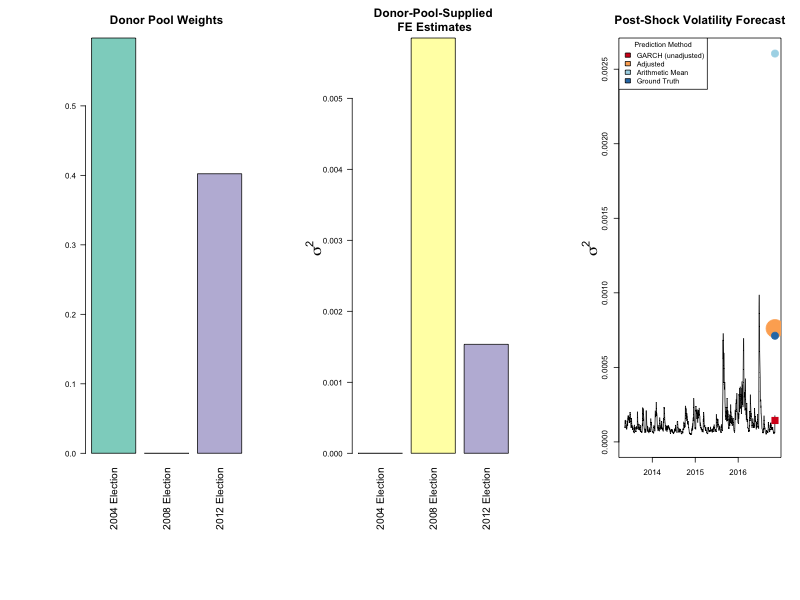
\includegraphics[scale=.34]{real_data_output_plots/savetime_SunMar172252462024_IYG_CL=F-^VIX-^IRX-^FVX-^TNX-^TYX_^VIX_2016-11-08-2004-11-02-2008-11-04-2012-11-06.png}
          \caption{The volatility induced by the 2016 US election}
          \label{fig:SVF_2016}
          \end{center}
        \end{figure}
\end{frame}

\section{Numerical Examples}

\begin{frame}{Hypotheses to Test Via Simulations}
    Ceteris paribus...
    \begin{enumerate}
        \item <1-> Distance-based weighting should \textcolor{red}{outperform} the unadjusted forecast as $\textcolor{blue}{\delta}$ increases (signal-to-noise)
        \item <2-> Distance-based weighting should \textcolor{red}{underperform} as the variability in $\textcolor{blue}{u_{i,t}}$ increases (signal-to-noise)
        \item <3-> Distance-based weighting should \textcolor{red}{outperform} the arithmetic mean as the variability of $\textcolor{blue}{\textbf{v}_{i,T^{*}}}$ increases between donors (importance of linear signal)
        \item <4-> Distance-based weighting should \textcolor{red}{underperform} the arithmetic mean as $\textcolor{blue}{\mu_{\omega^{*}}}$ increases (importance of linear signal)
        \item <5-> When $D^{return}_{i,T^{*}+1} = 1 = D^{vol}_{i,T^{*}+1}$, i.e. when there is both a \textcolor{red}{return shock} and \textcolor{red}{volatility shock}, our adjustment methods should \textcolor{red}{underperform} due to failed identification in $a_{T^{*}+1} = \sigma_{T^{*}+1}\epsilon_{T^{*}+1}$
    \end{enumerate}
\end{frame}

\begin{frame}
\fontsize{8pt}{9pt}

\frametitle{Simplest Simulation Setup}

Most elementary simulation regime tests Hypothesis 1 and 2 by varying $\textcolor{blue}{\delta}$ and $\textcolor{blue}{u_{i,t}}$.\\

\bigbreak

Recall an \hyperlink{model_1}{$\mc{M}_1$} model on the volatility, which is characterized by an exogenous shock to the volatility equation generated by an affine function of the covariates:

  \begin{align*}
    \mc{M}_1 \colon \begin{array}{l}
       \sigma^{2}_{i,t} = \omega_{i} + \omega^{*}_{i,t} + \sum^{m_{i}}_{k=1}\alpha_{i,k}a^{2}_{i,t-k} + \sum_{j=1}^{s_{i}}\beta_{i,j}\sigma_{i,t-j}^{2} + \gamma_{i}^{T} \x_{i,t} \text{ }\\[.2cm]
       a_{i,t} = \sigma_{i,t}((1-D^{return}_{i,t})\epsilon_{i,t} + D^{return}_{i,t}\epsilon^{*}_{i})\\[.2cm]
      \omega_{i,t}^{*} = D^{vol}_{i,t}[\mu_{\omega^{*}}+\textcolor{blue}{\delta}'\textbf{v}_{i, t}+ \textcolor{blue}{u_{i,t}}]\\[.2cm]
      D^{return}_{i,t} \equiv 0
    \end{array}
    \end{align*}

% https://www.overleaf.com/learn/latex/Beamer_Presentations%3A_A_Tutorial_for_Beginners_(Part_3)%E2%80%94Blocks%2C_Code%2C_Hyperlinks_and_Buttons
\end{frame}

\begin{frame}
    \fontsize{8pt}{9pt}
    
    \begin{figure}[h!]
      \begin{center}
        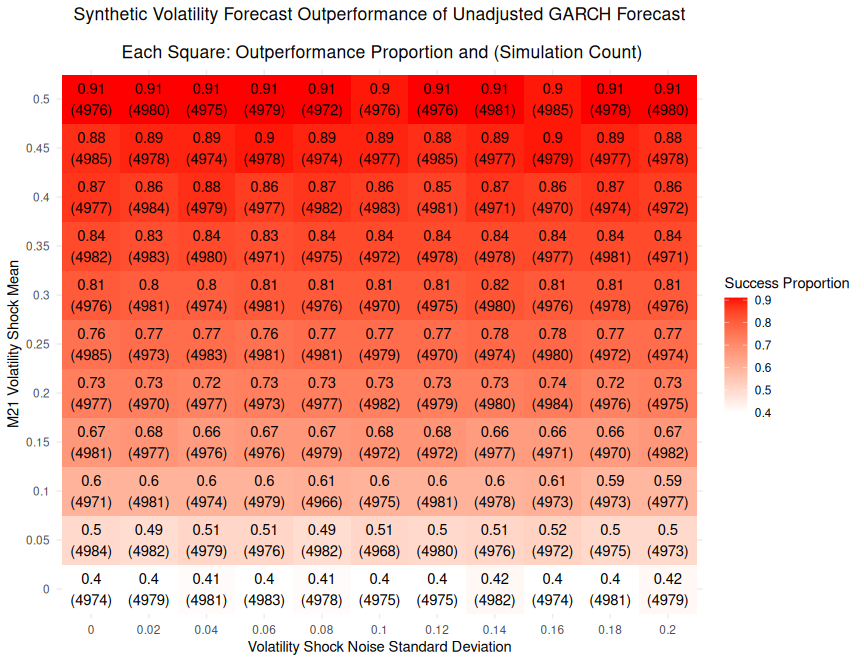
\includegraphics[scale=.29]{simulation_plots/standard_simulation_alpha_.1_beta_.82.png}
        \caption{Fixed parameter values: $\alpha = .1, \beta = .82, \mu_{x} = 1, \sigma_{x} = .1$}\label{fig:heavy_beta}
      \end{center}
      \end{figure}

\end{frame}

\begin{frame}
    \fontsize{8pt}{9pt}

    If we switch the values of $\alpha$ and $\beta$, we see similar behavior. 
    \begin{figure}[h!]
      \begin{center}
        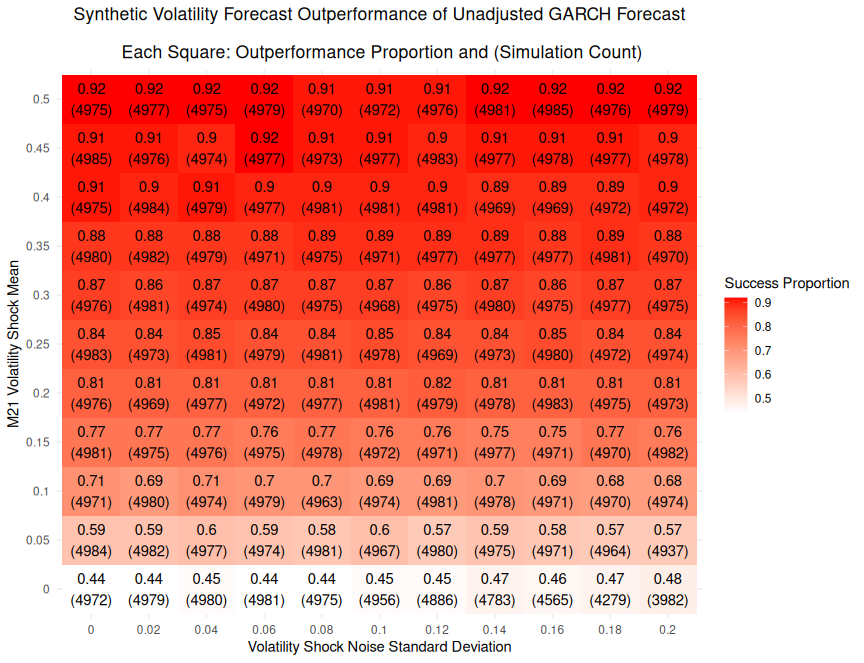
\includegraphics[scale=.29]{simulation_plots/standard_simulation_alpha_.82_beta_.1.png}
        \caption{Fixed parameter values: $\alpha = .82, \beta = .1, \mu_{x} = 1, \sigma_{x} = .1$}
        \label{fig:heavy_alpha}
      \end{center}
      \end{figure}

\end{frame}


\section{Future directions for Synthetic Volatility Forecasting}

\begin{frame}
We shall group the extensions into five buckets:
\begin{itemize}
    \item How much can we automate?
    \item Alternatives for fixed effect estimation
    \item Alternative estimators and estimands
    \item What can you do with a volatility forecast?
    \item Where else is distanced-based weighting useful?
\end{itemize}
\end{frame}

\begin{frame}{How much can we automate?}

Use NLP to identify donors.

\begin{figure}[H]
    \begin{center}
      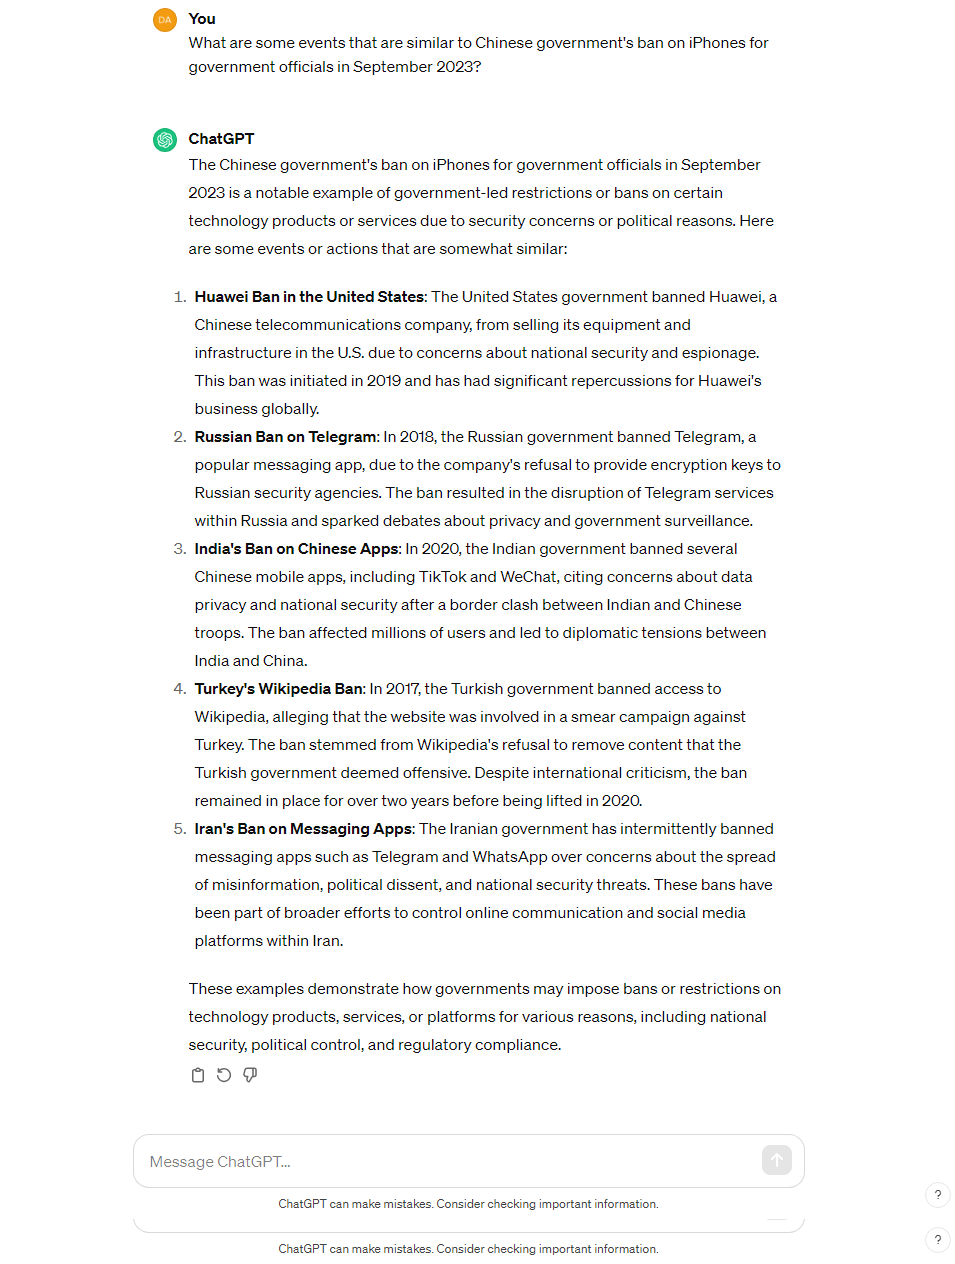
\includegraphics[scale=.18]{iphone.png}
      \end{center}
    \end{figure}


\end{frame}

\begin{frame}{How much can we automate?}

    What if the variables in the volatility profile are difficult to specify?

    \bigbreak
    Proposed solution:

    \bigbreak

    Use shrinkage estimation to detect fleeting signals in the cross section of $a_{t}^{2}$ \parencite[][]{chinco2019sparse}. 
\end{frame}

\begin{frame}
\frametitle{Alternative Ways of Estimating Fixed Effects}
High-frequency data?

\begin{itemize}

\item{Realized GARCH with High-Frequency Data}

\item{Stochastic Volatility}
\end{itemize}
\end{frame}

\begin{frame}
    \frametitle{Alternative Estimators and Estimands in Volatility Modeling}
    \begin{itemize}
        
        \item Factors in volatility profile
        \item Overnight returns instead of open-to-close
        
        \item Signal Recovery Perspective \parencite{ferwana2022optimal}
        
        \item Stochastic Volatility: Correlation between errors
        \item Multivariate GARCH
        
        \end{itemize}
\end{frame}

\begin{frame}
    \frametitle{What can you do with a volatility forecast?}
    \begin{itemize}
        \item{Value-at-Risk using SVF-based $\hat\sigma^{2}_{t}$}
        \end{itemize}
\end{frame}

\begin{frame}
    \frametitle{New Frontiers in Distance-based Weighting}
    \begin{itemize}
        \item Integrate lessons from literature on under/over reactions to information shocks \parencite[][]{jiang2017information}
        \item{Synthetic Impulse Response Functions}
        \end{itemize}
\end{frame}

\begin{frame}{Synthetic Impulse Response Functions: A Proposal}
    Suppose 
    \begin{itemize}
        \item We have a collection of $p$-variate time series of lengths $T_{i}, i=1,2,...n+1)$.
        \item We are interested in the response of variable $r$ to shocks in variable $j$, $1\leq r \leq j \leq p$. 

    \end{itemize}
    
\bigbreak
There many ways to estimate $IRF_{1}(r,j).$

\bigbreak
Can we somehow aggregate the estimates $\widehat{IRF}_{i}(r,j)$, $i = 2,3,...,n+1$? \\

Additional research questions:
\begin{itemize}
    \item What DGP would best motivate/justify such a method?
    \item Which method of IRF estimation would perform best?

\end{itemize}
\end{frame}
\section{Supplement}
We analyze the real data example with Brexit included.

\begin{figure}[H]
    \begin{center}
      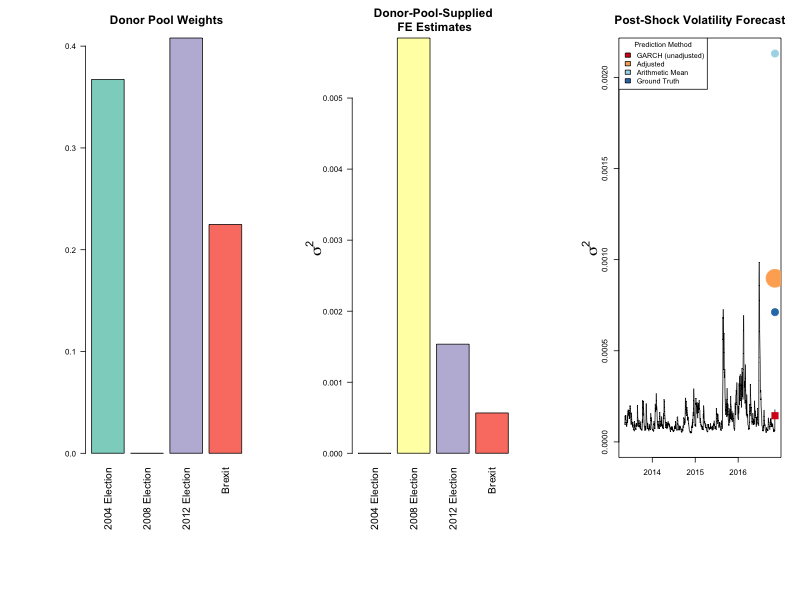
\includegraphics[scale=.32]{real_data_output_plots/savetime_SunMar172251232024_IYG_6B=F-CL=F-^VIX-^IRX-^FVX-^TNX-^TYX_^VIX_2016-11-08-2004-11-02-2008-11-04-2012-11-06-2016-06-22.png}
      \end{center}
    \end{figure}
    

\begin{frame}[t,allowframebreaks]
    \frametitle{References}
    % https://latex.org/forum/viewtopic.php?t=13344
    % \bibliographystyle{plainnat}
    % \bibliography{synthVolForecast}

\printbibliography[heading=none]
\end{frame}

\end{document}